\documentclass[conference]{IEEEtran}


%\usepackage{booktabs}
\usepackage{amsfonts}
\usepackage{nicefrac}
%\usepackage{microtype}


\usepackage[utf8]{inputenc}
\usepackage[T1]{fontenc}
\usepackage{lmodern}

\usepackage{algpseudocode}
\usepackage{algorithm}
%\usepackage{fixltx2e}
\MakeRobust{\Call}

% \usepackage{array}
%\usepackage{hyperref}

\usepackage[cmex10]{amsmath}
\usepackage{amssymb}
\usepackage{amsthm}
\DeclareMathOperator*{\argmax}{arg\,max}
\DeclareMathOperator{\similarity}{similarity}
\newtheorem{theorem}{Theorem}

%\usepackage{flushend}

\usepackage{xcolor}
\newcommand{\note}[1]{{\color{red}{#1}}{}}


%\usepackage{subfig}
\usepackage{graphicx}
\graphicspath{ {./figures/} }

\usepackage{tabularx}
% \usepackage{multirow}

% PSTRICKS drawing
% \usepackage[usenames,dvipsnames]{pstricks}
% \usepackage{epsfig}
% \usepackage{pst-grad} % For gradients
% \usepackage{pst-plot} % For axes
% \usepackage[space]{grffile} % For spaces in paths
% \usepackage{etoolbox} % For spaces in paths
% \makeatletter % For spaces in paths
% \patchcmd\Gread@eps{\@inputcheck#1 }{\@inputcheck"#1"\relax}{}{}
% \makeatother

% To add space before and after tables
%\usepackage{stackengine}

\setlength\parindent{0pt}
\setlength{\parskip}{4pt}%

\usepackage{caption} 
\captionsetup[table]{skip=5pt}


\usepackage{numprint}
\npthousandsep{\,}

\begin{document}

\title{Graph-based APT detection}

\author{
  \IEEEauthorblockN{Thibault Debatty}
  \IEEEauthorblockA{Royal Military Academy\\
  Belgium\\
  thibault.debatty@rma.ac.be}
  \and
  \IEEEauthorblockN{Wim Mees}
  \IEEEauthorblockA{Royal Military Academy\\
  Belgium\\
  wim.mees@rma.ac.be}
  \and
  \IEEEauthorblockN{Thomas Gilon}
  \IEEEauthorblockA{Royal Military Academy\\
  Belgium\\
  thomas.gilon@mil.be}
}


\IEEEoverridecommandlockouts\IEEEpubid{\makebox[\columnwidth]{978-1-5386-4559-8/18/\$31.00~\copyright~2018 IEEE \hfill} \hspace{\columnsep}\makebox[\columnwidth]{ }}



\maketitle

\begin{abstract}
In this paper we propose a new algorithm to detect Advanced Persistent Threats (APT's) that relies on a graph model of HTTP traffic. We also implement a complete detection system with a web interface that allows to interactively analyze the data. We perform a complete parameter study and experimental evaluation using data collected on a real network. The results show that the performance of our system is comparable to currently available antiviruses, although antiviruses use signatures to detect known malwares while our algorithm solely uses behavior analysis to detect new undocumented attacks.
\end{abstract}

\section{Introduction}

Advanced Persistent Threats (APT) are targeted cyber
attacks committed over a long period of time by highly
skilled attackers.

An example of an APT is the Miniduke attack~\cite{miniduke} that
targeted the governments of at least 20 countries including
the Czech Republic, Ireland, Portugal, Romania and the United States. The malware 
infected PCs when victims opened a cleverly
disguised Adobe PDF attachment to an email, which
was specifically tailored to the target. The attachment
referred to highly relevant subjects like foreign policy,
a human rights seminar, or NATO membership plans.

Such attacks are becoming evermore sophisticated
and manage to bypass the state of the art 
commercial-off-the-shelf protections that are currently in place.
The attackers regularly succeed in remotely controlling
hosts in our networks long enough to locate the information
they are after, gain access to it and finally
exfiltrate sensitive data. APT attacks have therefore
become a major concern for network security professionals
around the world.

All APT's have some characteristics in common. First, they use advanced techniques like 0-day attacks and social engineering to infect the target organization. This makes them impossible to detect using regular, signature based, detection tools like antiviruses and intrusion detection systems (IDS).

Second, once a computer is infected, an APT will try to establish a communication channel with a command and control (C2) server outside the organization. This channel will be used to download a payload, to download further instructions or to exfiltrate data. This link can be established using any protocol allowed through the borders of the organization: HTTP, DNS, SMTP, or even SIP.

In a security conscious organization, however, all these protocols should take place through some sort of choke-point. For the HTTP protocol, this would be a proxy server installed in the DMZ. This allows to log all connections taking place with servers located outside the organization, and offers a chance to detect the activity of the APT.

In this paper, we focus on the detection of APT's that use the HTTP protocol to establish a communication channel with their C2 server. Naive APTs perform connections to their C2 server at fixed or variable time intervals. This results in traces in the proxy logs that are quite easy to detect, like on top of Figure~\ref{fig:traffic}. The most evolved APT's however are able to sense user activity and wait for outgoing traffic to perform connections to the C2 servers. This makes them much more difficult to detect, like on the bottom of Figure~\ref{fig:traffic}. In this paper we focus on detecting the latter, activity-sensing APT's.

\begin{figure}
  \centering
  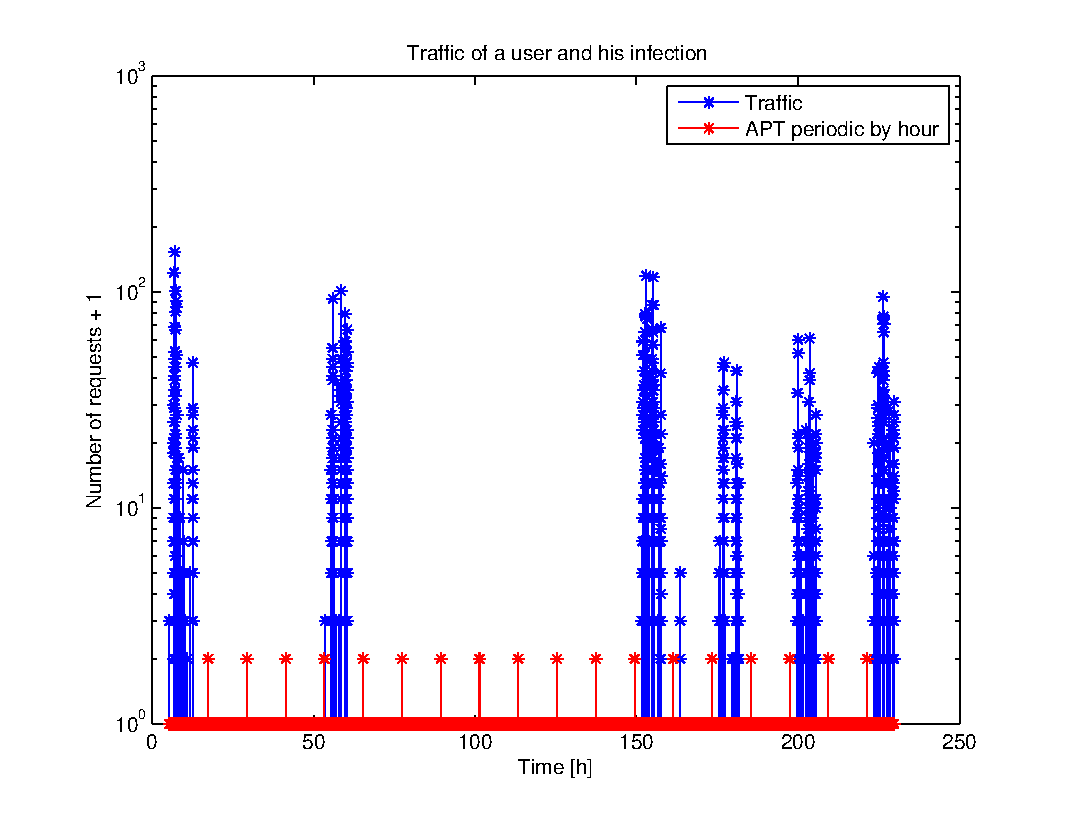
\includegraphics[width=0.9\linewidth]{traffic_perio.eps}
  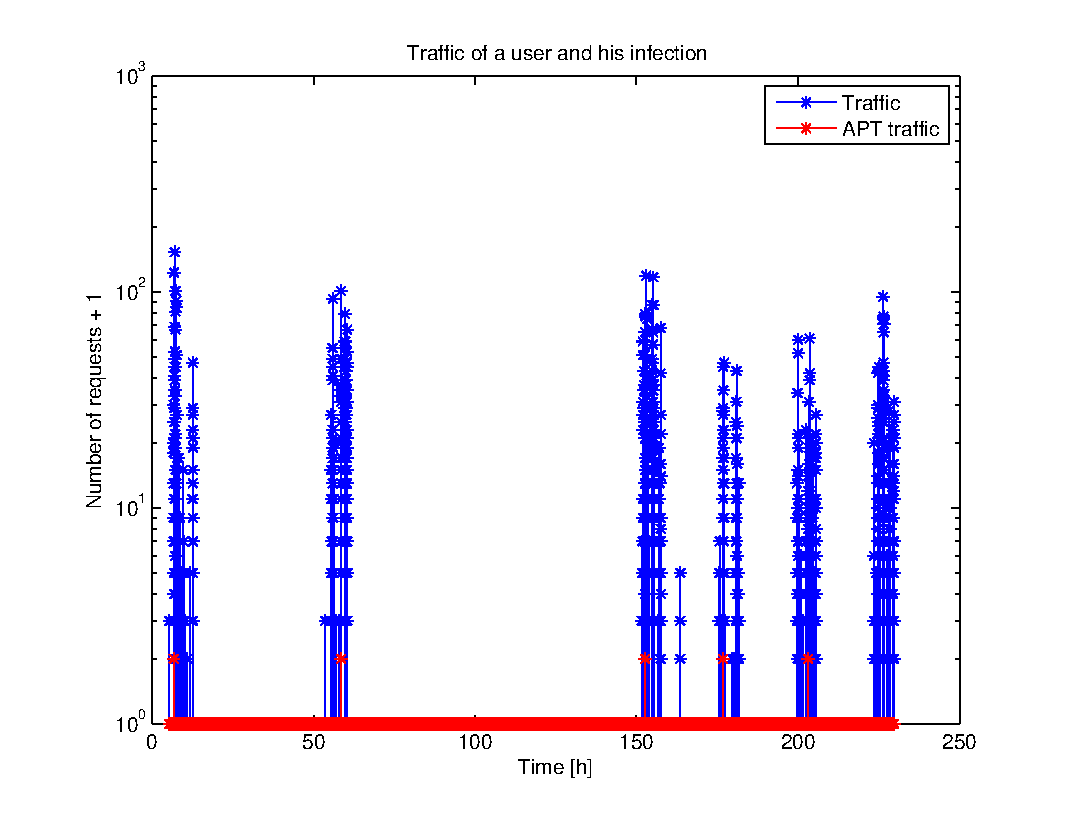
\includegraphics[width=0.9\linewidth]{traffic_traffic.eps}
  \caption{HTTP traffic generated by a single computer, infected by a frequency-based APT (top) and a sensing APT (bottom).}
  \label{fig:traffic}
\end{figure}

Therefore we build a graph of HTTP traffic. In this graph, the APT becomes an anomaly that can be detected. The rest of this paper is organized as follows: in Section~\ref{sec:model} we show how we model HTTP traffic, and we explain how this graph can be used to detect APT's; in Section~\ref{sec:implementation} we present how we implemented this algorithm in a complete detection system; in Section~\ref{sec:evaluation} we perform an experimental evaluation and we study the impact of the different parameters of the algorithm using data collected on a real network; finally, in Section~\ref{sec:conclusion} we present our conclusions.

\section{Graph modeling of HTTP traffic}
\label{sec:model}

\subsection{Modelization of legitimate traffic}

When a user is browsing the Internet, each page requested by the browser triggers multiple HTTP request. Usually, the first request contains HTML code, then the browser downloads javascript, CSS, font files and images referenced in the code. These may further trigger the download of other files, or trigger AJAX requests, and so on. Each page visited by a client can thus be represented by a tree, where the root is the original page requested by the user, and each subsequent request has a single edge (a link) to the request that triggered this download. These trees can be built from the logs of the proxy server. This is depicted on Figure~\ref{fig:tree}. The user successively opened three pages (pink, green and blue), which triggered a number of requests that can be observed in the logs of the proxy server.

\begin{figure}
  \centering
  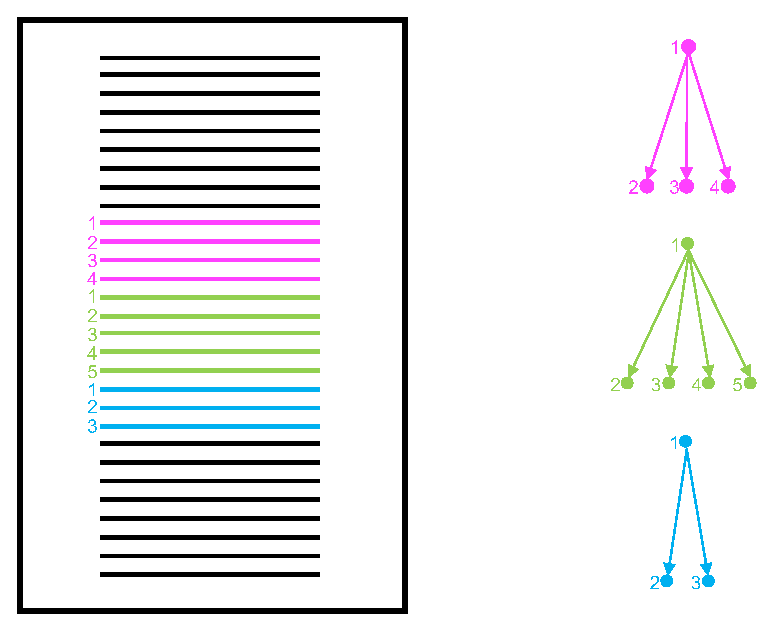
\includegraphics[height=85pt]{tree.eps}
  \caption{Graph model of HTTP traffic reconstructed from the logs of a proxy server}
  \label{fig:tree}
\end{figure}

In real-life, reconstructing the HTTP graph is much more complicated. First, requests belonging to multiple pages do frequently take place at the same moment. This can lead to the construction of incorrect trees. This is illustrated in Figure~\ref{fig:tree-multiple}.

\begin{figure}
  \centering
  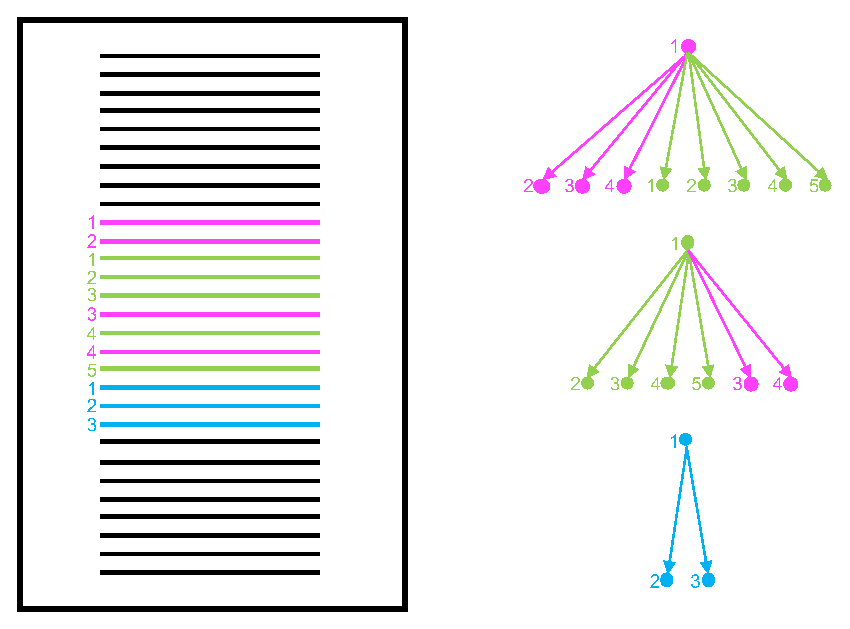
\includegraphics[height=85pt]{tree-multiple.eps}
  \caption{Graph model of HTTP traffic reconstructed from the logs of a proxy server when multiple pages are loaded in parallel.}
  \label{fig:tree-multiple}
\end{figure}

Second, as most pages on the Internet are built dynamically, loading the same page multiple times usually results in the execution of different, although similar, series of requests.

Finally, browsers try to keep in cache memory content that is not supposed to change, like images, javascript and css files. This also modifies the requests executed to display the same page.

Therefore we actually build a weighted graph, a graph where each node may have edges (links) to multiple other nodes, and each edge has a weight. In our graph, the weight of the edge from request $B$ to request $A$ indicates the probability that request $B$ is a consequence of request $A$. How we exactly compute these probabilities is explained below. Hence, a request (B) may have edges to multiple other requests, each indicating the probability that request A is a consequence of each other request.

\subsection{Detection of APT traffic}

When an APT waits for legitimate traffic (caused by a user browsing the Internet) to contact its C2 server, the requests performed by the APT take place roughly at the same moment as other requests from the graph. Hence, these requests have weak edges to multiple other requests.

This is illustrated in Figure~\ref{fig:tree-apt}: the requests performed by the APT happen together with the requests caused by the pink page, the green page and the blue page. As a consequence, the APT request has weak edges to all three root-requests.

\begin{figure}
  \centering
  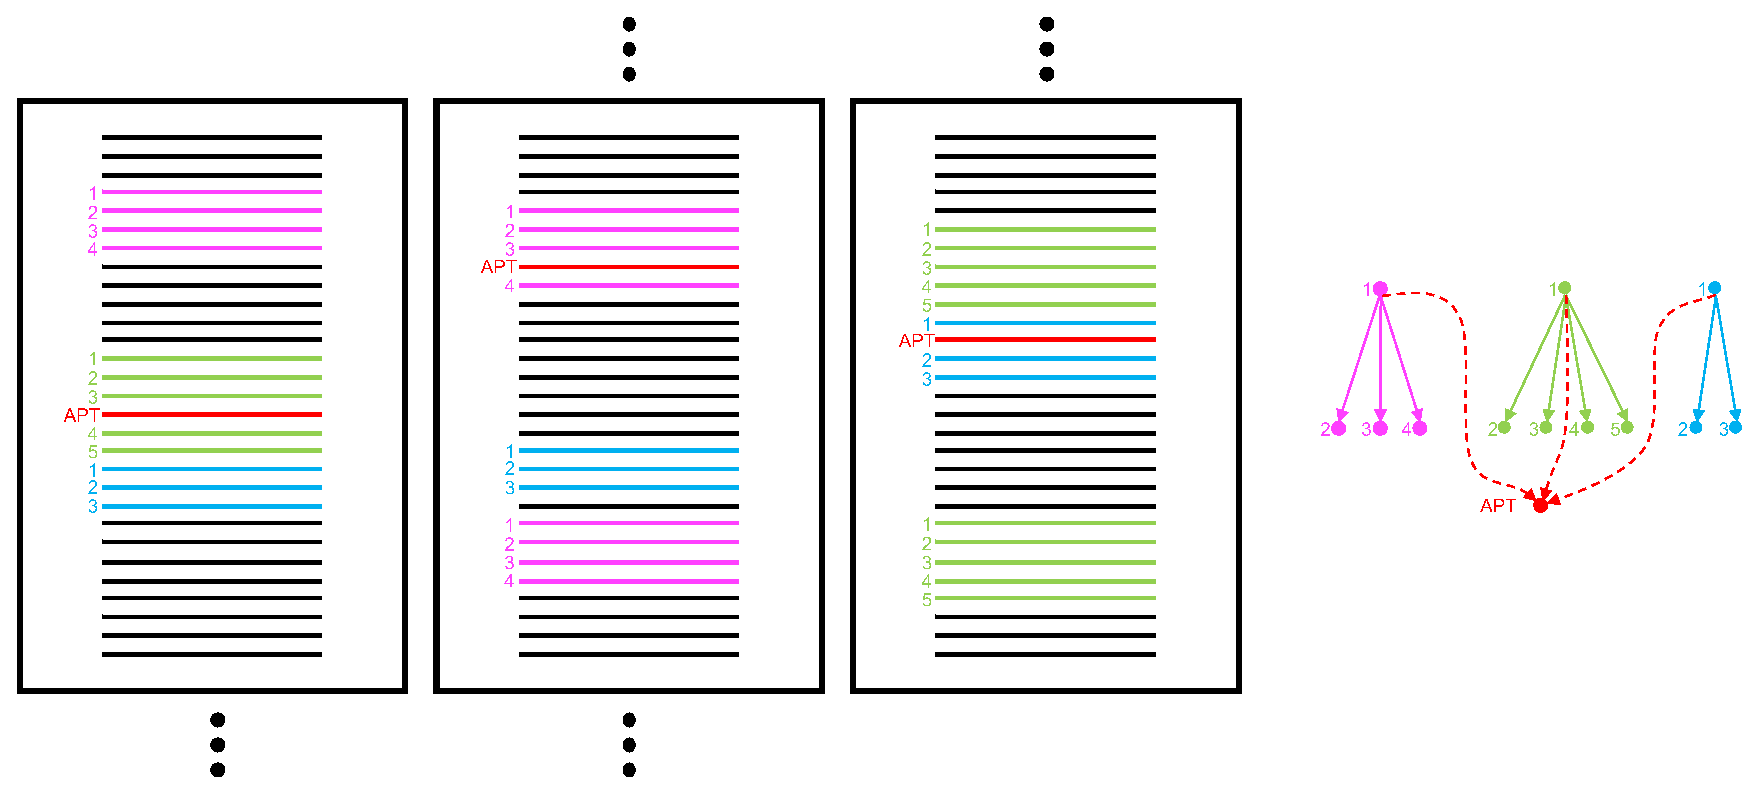
\includegraphics[height=100pt]{tree-apt.eps}
  \caption{Graph model of HTTP traffic reconstructed from the logs of a proxy server with the impact of a sensing APT.}
  \label{fig:tree-apt}
\end{figure}

A simple way to detect those requests is thus to prune the graph, which means to cut all edges whose value is lower then a threshold. The APT requests then appear as isolated nodes, while other legitimate requests are linked together into clusters.

\section{Implementation}
\label{sec:implementation}

To test the algorithm, we implemented a complete detection system\footnote{The complete source code and documentation are available at \texttt{https://github.com/RUCD/apt-graph}}. The system offers a web interface that allows the analyst to interactively analyze the requests taking place on the network using his browser. The detection relies on multiple parameters that the analyst can easily modify to spot hidden APT's. A screenshot of the web interface is presented in Figure~\ref{fig:ui}. This view was generated using log files from a real network, hence the domains were anonymized. APT's were simulated by injecting requests in the log.

\begin{figure*}
  \centering
  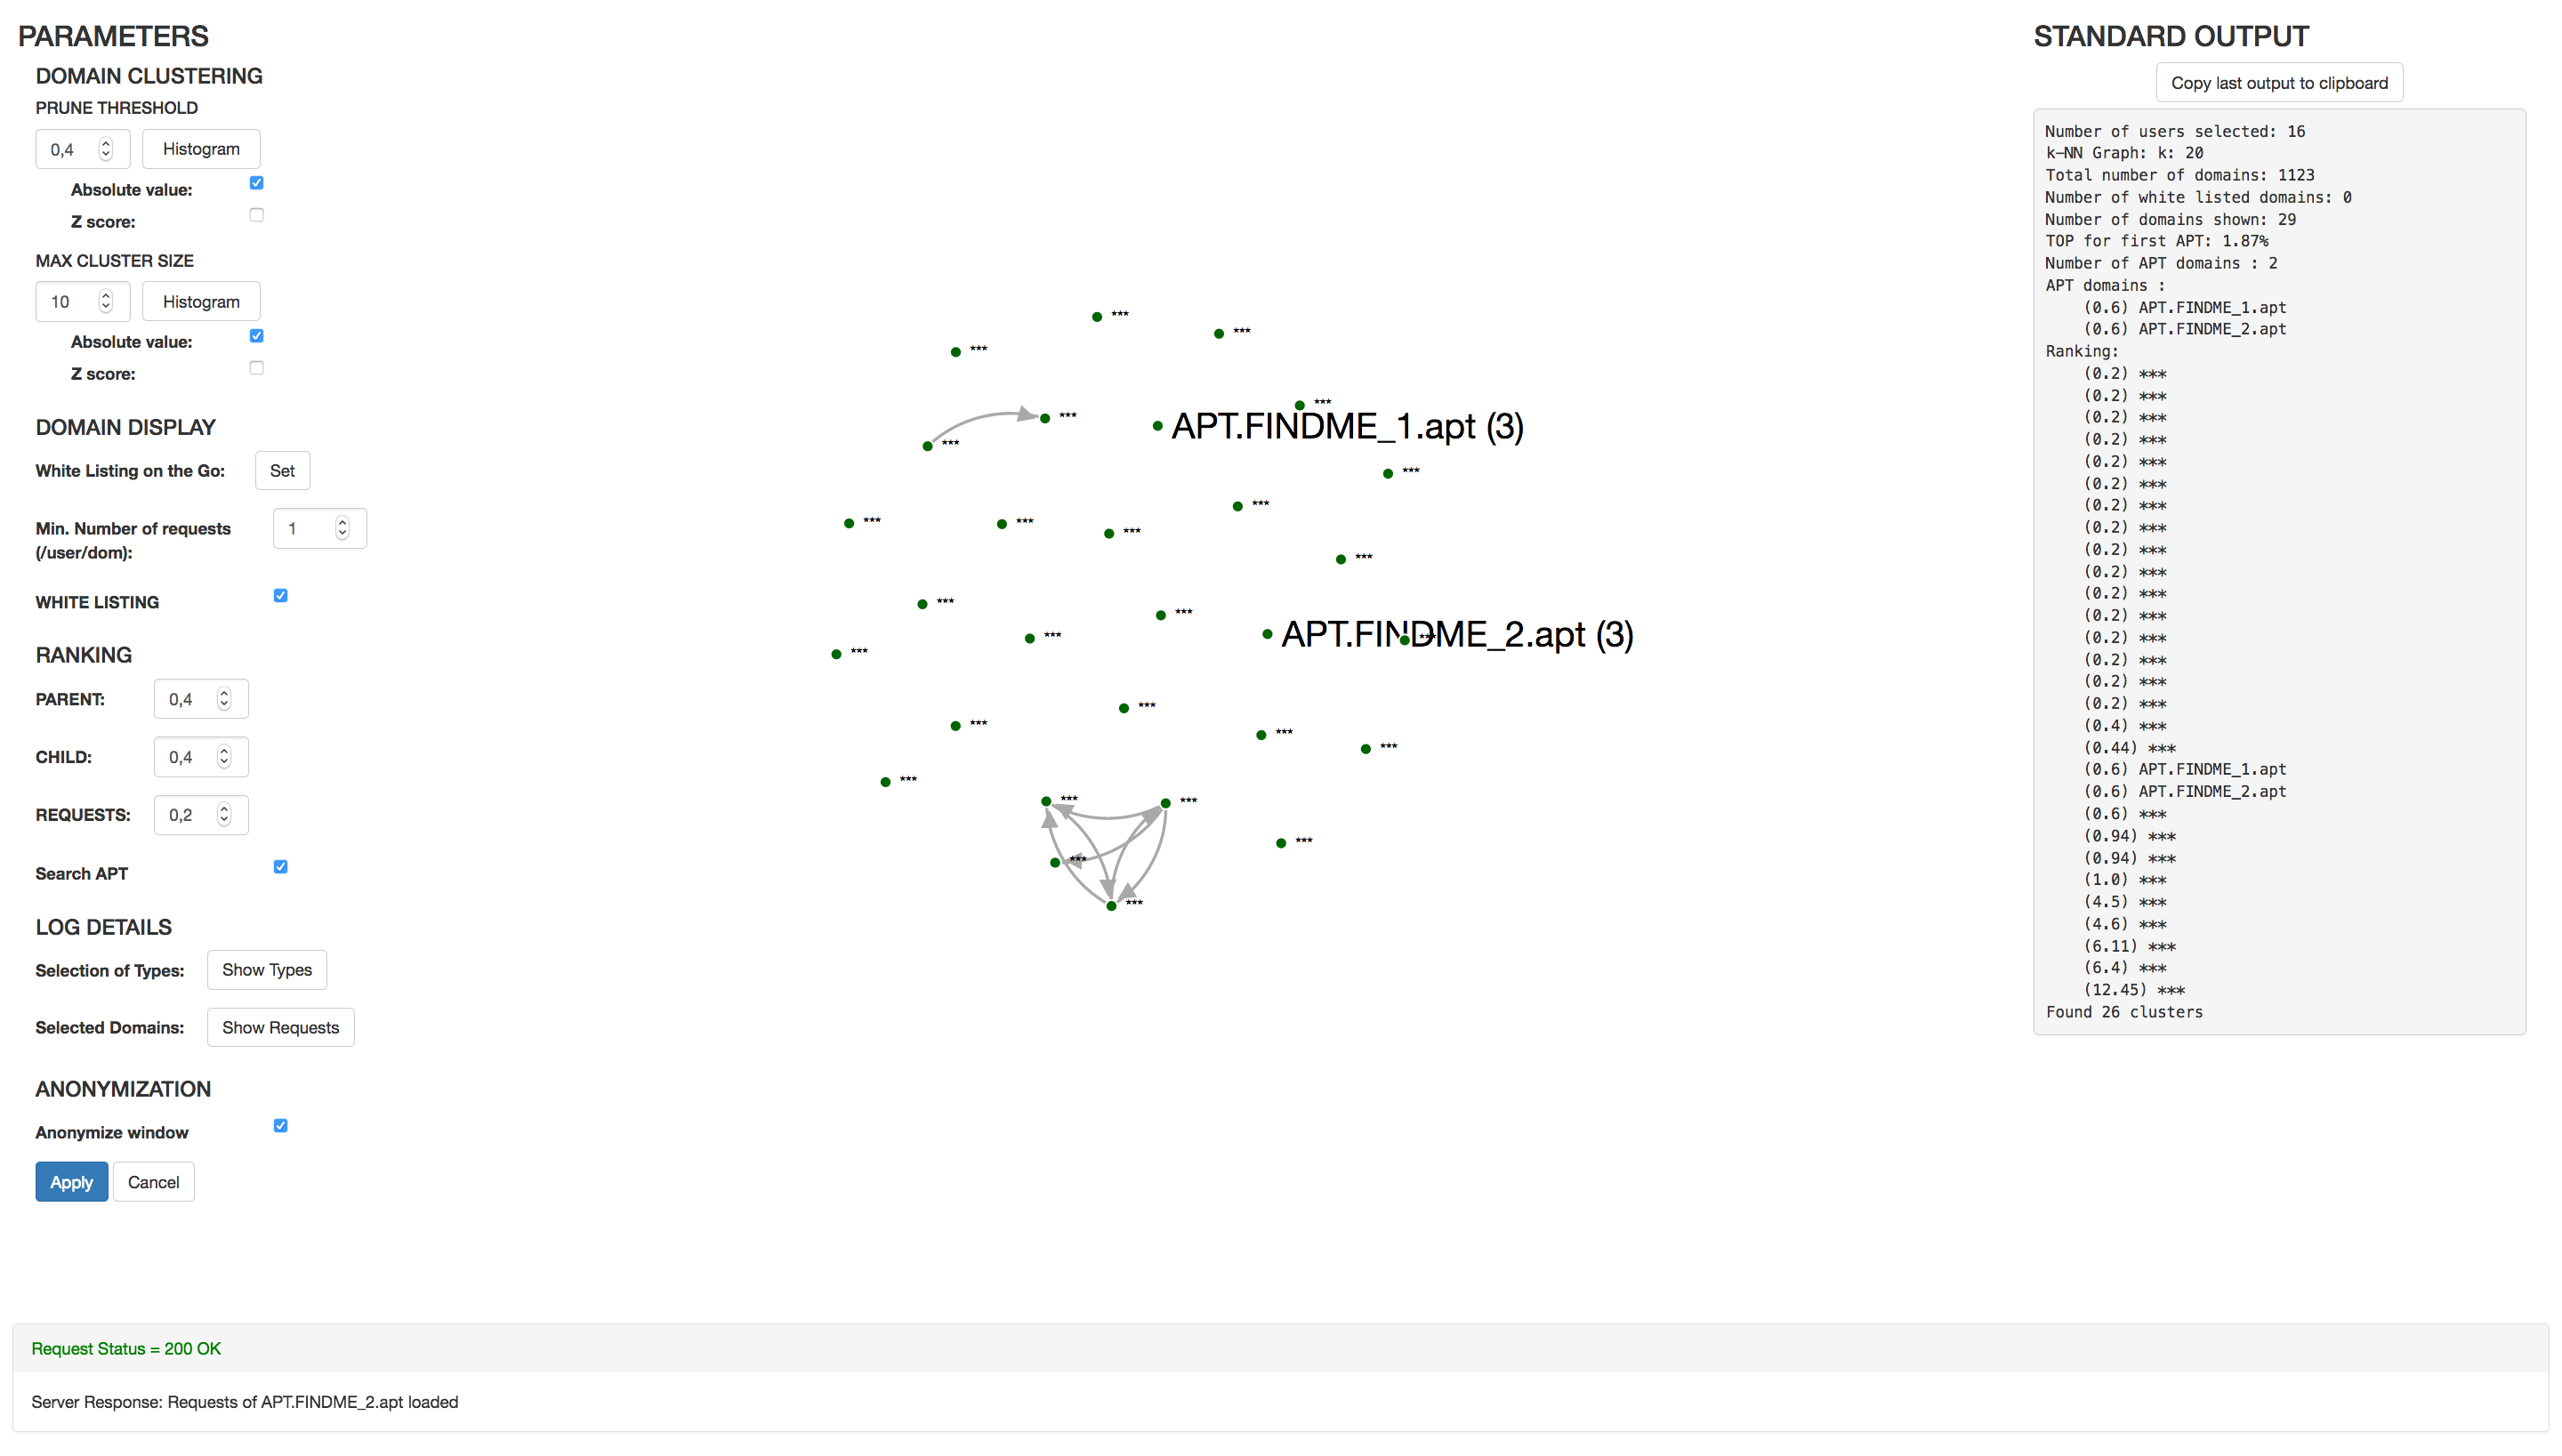
\includegraphics[width=1.0\linewidth]{ui.eps}
  \caption{Web interface of the detection system}
  \label{fig:ui}
\end{figure*}

The system consists in two components: 1) the batch processor and 2) the web interface that allows interactive analysis of the data.

\subsection{Batch processing}

The system is designed to allow the analysis of HTTP traffic generated by large networks of computers. In such networks, millions of requests are generated each day. Storing a complete (fully connected) graph requires to store $O(n^2)$ values, where $n$ is the number of nodes in the graph. Hence, storing a graph containing just 1 million requests requires roughly 1TB of storage. With current hardware, this is heavy to store on disk and almost impossible to store in memory unless a supercomputer is used. Hence, we instead build a $k$-nearest neighbors ($k$-nn) graph, a graph were each node has an edge to the $k$ most similar other nodes in the graph. These graphs are a close approximation of a complete graph if $k$ is large enough. However, they have the huge advantage that their memory requirement is linear in $n$ (namely $kn$), which makes them also faster to process~\cite{LulliDDMR15}.

Before the $k$-nn graph is stored, it has to be computed, which requires to compute $O(n^2)$ similarities using a naive algorithm. This is not acceptable either for the large graphs we envision. Hence we use instead a fast approximate algorithm called nn-descent that requires to compute $O(n^{1.14})$ similarities to build the $k$-nn graph~\cite{Dong2011}. Moreover, this algorithms can easily be implemented in parallel, which allows to take advantage of all the cores available on the processing server.

Even using theses two optimizations ($k$-nn graphs and nn-descent algorithm), building the graph is a computationally heavy process that requires a non-negligible amount of time. Hence the system is split in two separate components: a batch processor and a web interface to perform the analysis.

The batch processor is responsible for computing the initial graph, without applying any detection. As the name states, this time consuming processing is meant to be run only once for each dataset.

Moreover, the system is designed to let the analyst tweak the definition of similarity between requests. Indeed, multiple criteria can be used to measure the probability that request B is a consequence of request A:

\begin{itemize}
\item requests A and B belong to the same domain;
\item request B took place shortly after request A;
\item etc.
\end{itemize}

In a naive implementation, modifying the definition of similarity, even slightly, requires to recompute the complete $k$-nn graph. Once again, this is a time consuming operation that would not allow to interactively analyze the data. Instead, during batch processing, we compute multiple graphs: one for each elementary similarity.

The time graph is built using the following measure of similarity:

$$ \mu_{\text{time}} = \frac{1}{1+ |{\delta t}|}$$

where $\delta t$ is the time difference (in seconds) between two requests.

The domain graph, however, is built using following measure of similarity:

$$\mu_{\text{domain}} = \frac{\beta(A,B)}{\max(\gamma(A), \gamma(B))}$$

In this equation, $\beta(A,B)$ is the number of labels in common in the domain names of request $A$ and $B$, starting from the Top Level Domain (TLD), and excluding the TLD itself. For example, $\beta(\text{cnn.com}, \text{www.cnn.com}) = 1$ because they have the label "cnn" in common. $\gamma(A)$ is the number of labels in the domain name of A, without taking the TLD into account. For example, $\gamma(\text{www.cnn.com}) = 2$

%The complete processing chain is depicted in Figure~\ref{fig:batch-processing}.

%\begin{figure*}
%  \centering
%  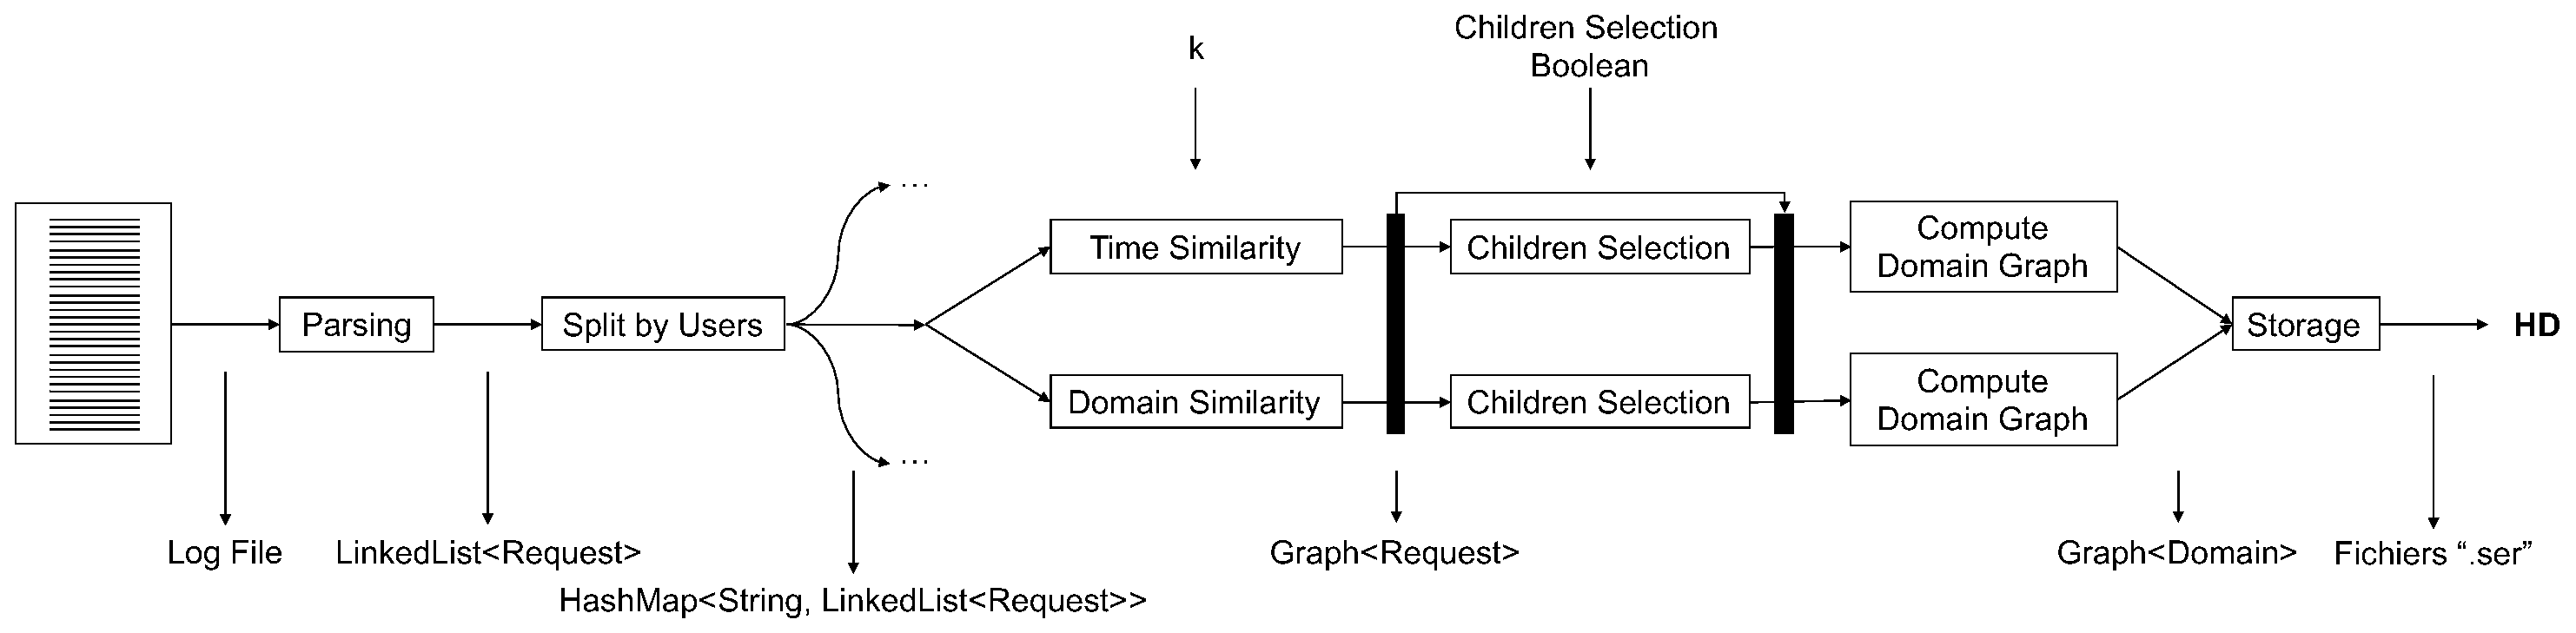
\includegraphics[width=1.0\textwidth]{batch-processing.eps}
%  \caption{Batch processing chain}
%  \label{fig:batch-processing}
%\end{figure*}

The complete batch processing thus involves the following steps:

\begin{itemize}
\item \textbf{Split} The data is first split between the different clients in the network, which corresponds to the "source IP" field in the proxy logs;
\item \textbf{Graphs} For each client, the different $k$-nn graphs are computed
\item \textbf{Domains} As we suspect the APT will use different URL's belonging to the same domain, the different requests from the same domain are merged together to build graphs of domains;
\item \textbf{Save} The graphs of domains are saved to disk.
\end{itemize}

The batch processor only takes one parameter, $k$, the number of edges per node in the $k$-nn graph. The impact of varying this parameter is shown below.

\subsection{Interactive analysis}

Once the batch processor has computed the $k$-nn graphs, these can be interactively analyzed using the web interface. The analysis mainly requires to: 1) merge the different $k$-nn graphs, 2) remove weak edges (pruning), 3) cluster the graph, 4) filter the graph to show only isolated domains and 5) rank the remaining suspicious domains.

In this process, the operator can provide several parameters to improve the detection.

First, he can choose which \textbf{clients} from the network are analyzed. Merging the graphs corresponding to multiple clients reinforces the edges between naturally related domains. This makes the domains contacted by the APT more isolated and hence easier to detect.

The analyst can also modify the definition of \textbf{similarity} used to link requests by providing a different weight for the time similarity and for the domain similarity.

He can provide a \textbf{pruning threshold} to remove weak edges from the the final graph. A high threshold removes a lot of edges in the graph, which leaves a lot of requests isolated. This causes a higher number of false positives. At the opposite, a lower value leaves almost all edges unaffected. Hence the requests generated by the APT have a higher probability of remaining connected to other requests, which decreases the probability of detection. The pruning threshold can be defined as an absolute value or as a z-score. The relation between a z-score $z$ and an absolute value $x$ is defined as follows:

$$ z = \frac{x - \mu}{\sigma} $$

Using z-scores allows to specify values that are independent of the data.

For the filtering step, the analyst can provide a \textbf{maximum cluster size}. Theoretically, after the pruning step the APT is supposed to be completely isolated. However, if the pruning threshold is chosen slightly too low, the APT may remain connected to some other domains, thus creating a small cluster. By using a filter to show only small clusters, the analyst may be able to spot the APT.

To further filter the results, the analyst can specify a \textbf{minimum number of requests per domain}. During our experimental evaluation with real data, we discovered that regular HTTP traffic contains a lot of domains that have very few requests each. Because they have very few requests, they are weakly connected to other domains, and are thus considered as suspicious by our system. An APT, however, has to regularly contact its C2 server to download further instructions or to exfiltrate data. Hence we give the analyst the possibility to filter out domains with very few requests.

Finally, the system performs a \textbf{ranking} of remaining suspicious domains. Therefore we use three parameters, with weights provided by the analyst: 1) the number of requests to this domain, as a stealthy APT is supposed to perform only a few requests, 2) the number of child domains in the graph and 3) the number or parent domains in the graph, as the domain used by an APT is supposed to be weakly connected to multiple other domains.

In summary, the following steps are executed to perform the analysis:

\begin{itemize}
\item \textbf{Load} The $k$-nn graphs are read from the disk;
\item \textbf{Feature fusion} The domain and time graphs are merged using the weights provided by the analyst;
\item \textbf{Users fusion} The graphs corresponding to the different users selected by the analyst are merged;
\item \textbf{Pruning} Weak edges are removed from the graph;
\item \textbf{Clustering};
\item \textbf{Filtering} Clusters larger then a threshold provided by the analyst are removed;
\item \textbf{Filtering} Domains that don't have enough requests are removed;
\item \textbf{Ranking} The remaining suspicious domains are sorted using weights provided by the analyst.
\end{itemize}

Although this may seem heavy, processing $k$-nn graphs is actually extremely fast. This allows to interactively analyze huge amounts of data.

\section{Parameter study and experimental evaluation}
\label{sec:evaluation}

\subsection{Test setup}

To test the system, we use the logs from the proxy server of real, large organization. From this huge dataset, we chose a subnet consisting of 26 computers, and a time period of 10 days. This subset contains a total of \numprint{721921} requests.

In this log file, requests are inserted to simulate the activity of 4 APT's in the network. These APT's are chosen to exhibit different typical behaviors. The least stealthy APT generates 239 requests to its C2 server while the most stealthy APT performs only 13 requests in total, which makes it very difficult to detect.

To test the quality of detection, we build the receiver operating characteristic (ROC) curve of the detection system: we generate a ranking of the requests according to their suspiciousness using the provided parameters set. Then we walk the list from the top, and we compare each request to the known list of requests performed by the APT's. At each level of the list, we compute the probability of detection ($p_d$) and probability of false alarm ($p_{fa}$):

$$p_d = \frac{\text{number of domains corresponding to an APT}}{\text{number of domains considered in the list}}$$

$$p_{fa} = \frac{\text{number of legitimate domains}}{\text{number of domains considered in the list}}$$

This allows to draw the ROC of the system, like depicted in Figure~\ref{fig:roc}.

\begin{figure}
  \centering
  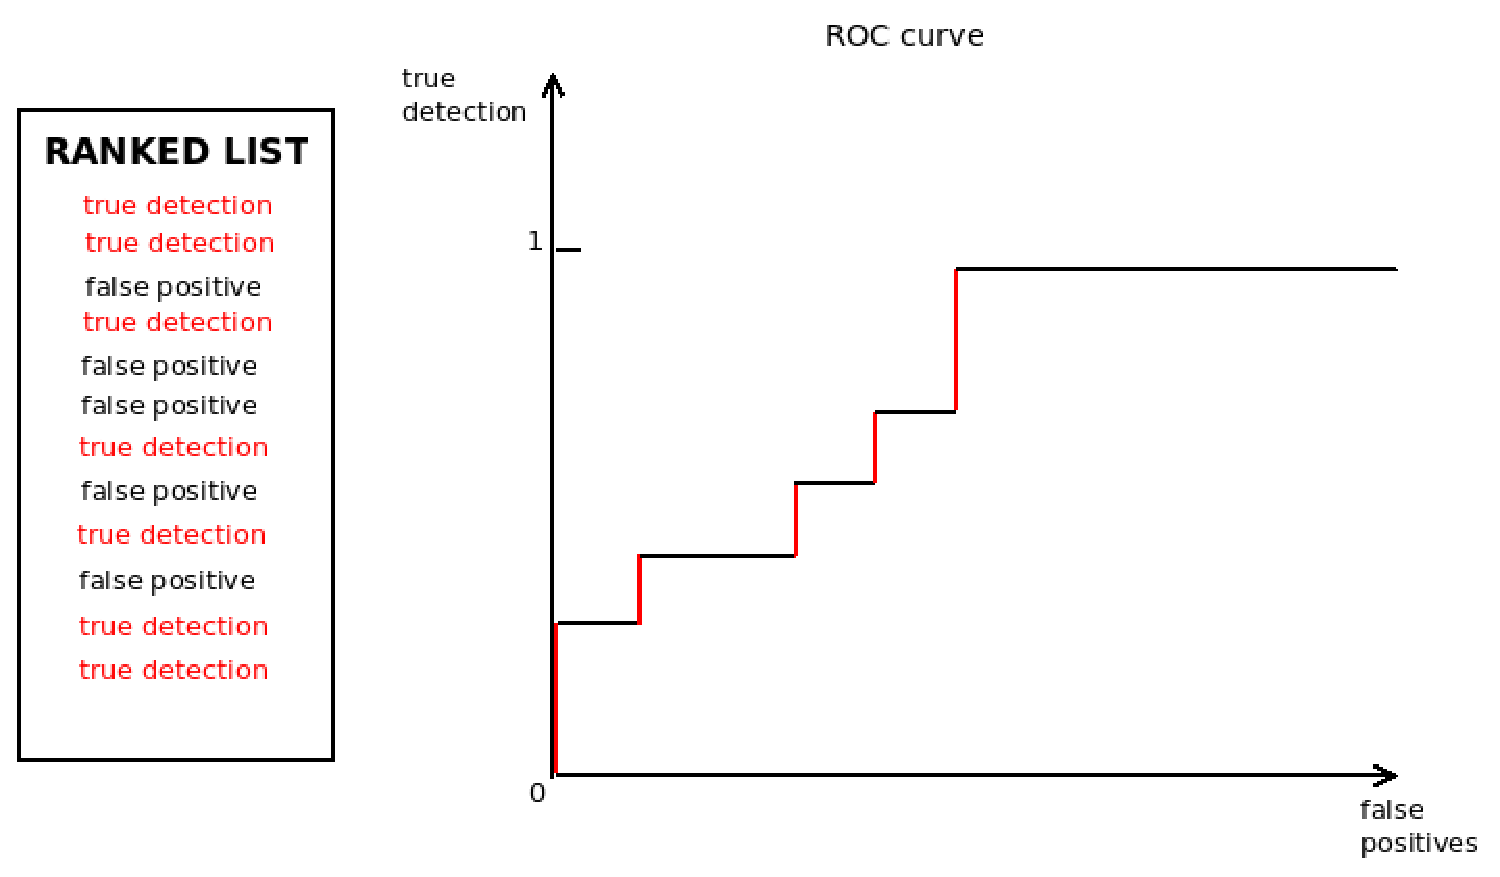
\includegraphics[width=1.0\linewidth]{bench_roc.eps}
  \caption{Building the receiver operating characteristic (ROC) curve of a detection system}
  \label{fig:roc}
\end{figure}

Finally, to compute the quality of the detection, we compute the area under the curve (AUC). Indeed, for a perfect detection system $p_d = 1 \ \forall \ p_{fa}$, hence $\text{AUC} = 1$. At the opposite, the worst detection system has $p_d = 0 \ \forall \ p_{fa}$, hence $\text{AUC} = 0$.

\subsection{Number of edges per node $k$}

For the first test, with vary values for $k$, the number of edges per node in the initial graphs.

We use the following values for the tests:

{\small
  \begin{tabularx}{\linewidth}{rl}
  \hline
  Weight time similarity & 0.5 \\ 
  Weight domain similarity & 0.5 \\ 
  Pruning (z-score) & 0.0 \\
  Filtering: max cluster size & $1000000$ \\ 
  Filtering: requests/domain/client & $1$ \\ 
  Ranking: weight parents & $0.35$ \\ 
  Ranking: weight children & $0.35$ \\ 
  Ranking: weight number of requests & $0.3$ \\
  \hline
  \end{tabularx}
}

The resulting ROC and AUC are presented on Figure~\ref{fig:test:k}.

Surprisingly, $k = 40$ seems to give better results then $k = 100$. To study this effect, we perform additional tests where we compare these two cases by varying the other parameters. The values used for the different tests are presented in Table~\ref{table:k} and the results are shown on Figure~\ref{fig:test:k:2}.

\begin{table*}
  \centering
  % &  &  &  &  &  &  &  &  &  &  \\
  \begin{tabular}{rcccccccccc}
  \hline
  Test & 1 & 2 & 3 & 4 & 5 & 6 & 7 & 8 & 9 & 10 \\ \hline
  k & 40 & 100 & 40 & 100 & 40 & 100 & 40 & 100 & 40 & 100 \\
  Weight time similarity & 0.1 & 0.1 & 0.4 & 0.4 & 0.1 & 0.1 & 0.1 & 0.1 & 0.1 & 0.1 \\ 
  Weight domain similarity & 0.9 & 0.9 & 0.6 & 0.6 & 0.9 & 0.9 & 0.9 & 0.9 & 0.9 & 0.9 \\ 
  Pruning (z-score) & 0.0 & 0.0 & 0.0 & 0.0 & -0.1 & -0.1 & -0.5 & -0.5 & 0.0 & 0.0 \\ 
  \hline
  Filtering: max cluster size & \multicolumn{10}{c}{1000000} \\ 
  Filtering: requests/domain/client & \multicolumn{10}{c}{5} \\ 
  \hline
  Ranking: weight parents & 0.4 & 0.4 & 0.4 & 0.4 & 0.4 & 0.4 & 0.4 & 0.4 & 0.5 & 0.5 \\ 
  Ranking: weight children & 0.4 & 0.4 & 0.4 & 0.4 & 0.4 & 0.4 & 0.4 & 0.4 & 0.5 & 0.5 \\ 
  Ranking: weight number of requests & 0.2 & 0.2 & 0.2 & 0.2 & 0.2 & 0.2 & 0.2 & 0.2 & 0.0 & 0.0 \\
  \hline
  \end{tabular}
  \caption{Parameters used to compare $k = 40$ and $k = 100$}
  \label{table:k}
\end{table*}

As we can see, although $k = 40$ does provide slightly better results in some cases, $k = 100$ is generally better, as we expected. From now on, we use $k = 100$ for all our tests.

\subsection{Fusion weights}

We now study the impact of varying the weights used to merge the graph built using time similarity and the graph built using domain similarity. To perform the test, we have to fix a value for all other parameters. Therefore we choose neutral values, even though we now these are suboptimal. For example, we use a large value for the maximum cluster size, such that we don't filter clusters out:

{\small
  \begin{tabularx}{\linewidth}{rl}
  \hline
  k & 100 \\
  Pruning (z-score) & 0.0 \\
  Filtering: max cluster size & $1000000$ \\ 
  Filtering: requests/domain/client & $1$ \\ 
  Ranking: weight parents & $0.35$ \\ 
  Ranking: weight children & $0.35$ \\ 
  Ranking: weight number of requests & $0.3$ \\
  \hline
  \end{tabularx}
}

The results are shown on Figure~\ref{fig:test:weights}.

The best result is achieved when the weight for time based similarity is $0.1$ and the weight for domain based similarity is $0.9$. This shows that the fact that two requests belong to the same domain is a better indicator of the link between the requests than the fact that these two requests happen slightly at the same moment. This was expected, as APT's wait for activity to contact their C2 servers. From now on we use these values for other tests.

\subsection{Pruning}

We now vary the pruning threshold. To keep the test independent of the data, we actually vary the z-score of the pruning threshold. The other parameters used for the test are:

{\small
\begin{tabularx}{\linewidth}{rl}
\hline
$k$ & 100 \\
Weight time similarity & 0.1 \\ 
Weight domain similarity & 0.9 \\
Filtering: max cluster size & $1000000$ \\ 
Filtering: requests/domain/client & $1$ \\ 
Ranking: weight parents & $0.35$ \\ 
Ranking: weight children & $0.35$ \\ 
Ranking: weight number of requests & $0.3$ \\
\hline
\end{tabularx}
}

The results are shown on Figure~\ref{fig:test:pruning}.

\subsection{Size of clusters}

Now we vary the maximum size of clusters using following parameters:

{\small
\begin{tabularx}{\linewidth}{rl}
\hline
$k$ & 100 \\
Weight time similarity & 0.1 \\ 
Weight domain similarity & 0.9 \\
Pruning (z-score) & 0.0 \\
Filtering: requests/domain/client & $1$ \\ 
Ranking: weight parents & $0.35$ \\ 
Ranking: weight children & $0.35$ \\ 
Ranking: weight number of requests & $0.3$ \\
\hline
\end{tabularx}
}

The results are presented on Figure~\ref{fig:test:cluster}. Interestingly, the best result is obtained when the maximum cluster size is \numprint{1000.000}, which shows that even after pruning, the APT's are usually still linked to some much larger clusters. 

\subsection{Minimum number of requests per client}

This parameter is studied using the setup:

{\small
\begin{tabularx}{\linewidth}{rl}
\hline
$k$ & 100 \\
Weight time similarity & 0.1 \\ 
Weight domain similarity & 0.9 \\
Pruning (z-score) & 0.0 \\
Filtering: max cluster size & 1000000 \\
Ranking: weight parents & $0.35$ \\ 
Ranking: weight children & $0.35$ \\ 
Ranking: weight number of requests & $0.3$ \\
\hline
\end{tabularx}
}

The results are presented in Figure~\ref{fig:test:requests}.

As we explained above, filtering out the domains that receive very few requests per day (less then 5) allows to drastically reduce the background "noise" and improves the quality of detection.

\subsection{Ranking weights}

We now vary the weights used to perform the ranking of remaining domains. We use the following parameters:

{\small
  \begin{tabularx}{\linewidth}{rl}
  \hline
  $k$ & 100 \\
  Weight time similarity & 0.1 \\ 
  Weight domain similarity & 0.9 \\
  Pruning (z-score) & 0.0 \\
  Filtering: max cluster size & 1000000 \\
  Filtering: requests/domain/client & $5$ \\
  \hline
  \end{tabularx}
}

We first vary the weight of the number of requests, and set the two other weights accordingly:

\begin{equation*}
\begin{split}
 \frac{1 - \text{weight number of requests}}{2} \\
    & = \text{weight number of children} \\
    & = \text{weight number of parents}
\end{split}
\end{equation*}

The results are shown in Figure~\ref{fig:test:ranking}.

Using a negative value for the number of requests seems to provide the best results. However, this also first enlightens the less stealthy APT's, that perform a lot of requests to their C2 servers. Hence we recommend here to use a slightly positive value, namely $0.2$.

\subsection{Cross validation}

We have now identified the parameters that seem to offer the best quality of detection. These parameters must of course be tuned by the analyst for the network under test, and for the kind of APT he tries to detect on the network (is the APT supposed to be more or less stealthy, etc.). However, we assume these are robust enough to represent a relevant starting point for the analyst.

To test this hypothesis, we use another subnet of the proxy log. This time, the subnet contains 66 clients, 10 days of data and \numprint{1032021} requests. We simulate the infection with 8 APT's and we analyze the data with the optimal parameters identified previously.

The resulting ROC is presented in Figure~\ref{fig:test:cross} and has an AUC of $0.9036$. This shows the algorithm is very resilient and performs equally well with a different dataset. It also shows that the system quickly discovers 90\% of the APT's. This is equivalent to the performance of most antiviruses on the market, with the huge difference that antiviruses use signatures to detect known malwares, while our detector solely uses behavior analysis to detect new undocumented attacks.

\subsection{Detected domains}

As we stated above, the dataset used to perform the tests is produced from the logs of the proxy server of a real network. Hence we manually analyzed the domains that were ranked as APT's by the system. These are mainly:

\begin{itemize}
  \item Content Delivery Networks (CDN);
  \item domains that display advertising on multiple websites;
  \item domains that deliver Javascript libraries to multiple websites;
  \item websites with very few visits.
\end{itemize}

Although these are not C2 servers per se, they are characterised by the same behavior as the APT's that we are trying to detect: they weak links with a lot of other requests. This shows that the algorithm is actually performing very well at detecting domains that behave like the domains used by an APT to contact its C2 server.

\section{Conclusion and future work}
\label{sec:conclusion}

The results obtained by our detection algorithm are very promising as they do not rely on a previous knowledge of the attacks. As a future work we plan to further tune the detection parameters using deep learning, to further improve the quality of detection.


\bibliographystyle{IEEEtran}
\bibliography{paper}

\begin{figure}
  \centering
  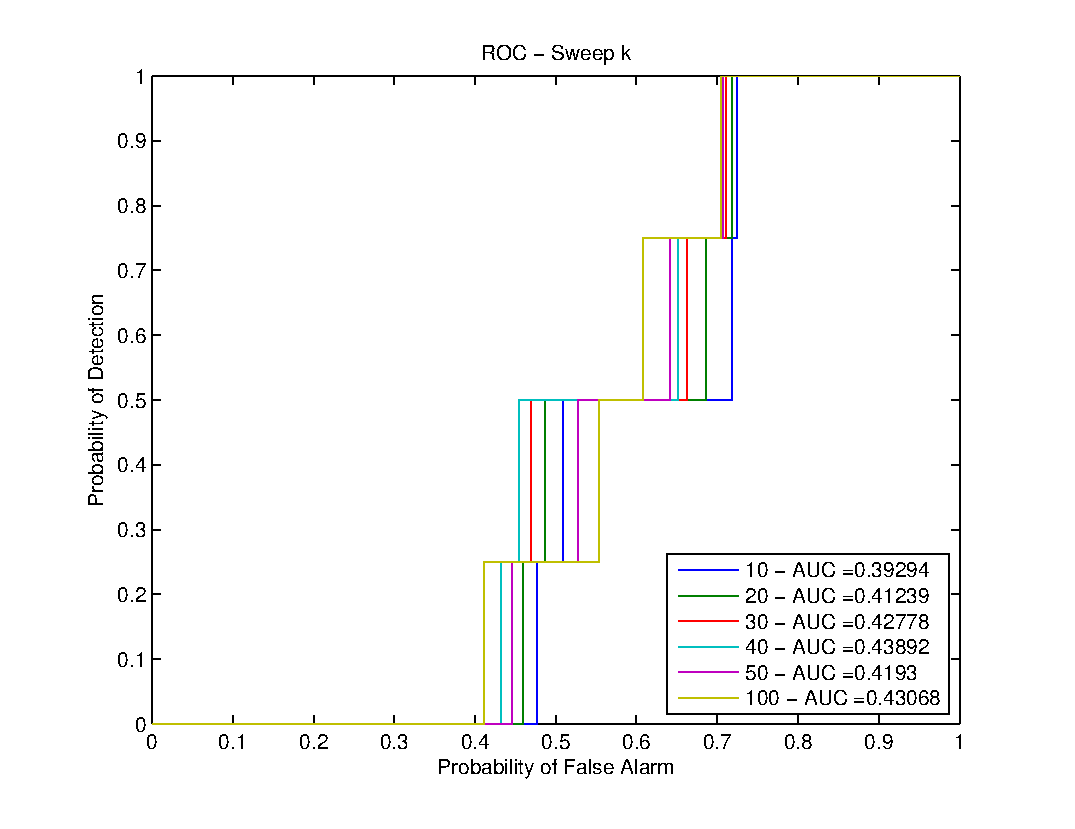
\includegraphics[width=0.9\linewidth]{k_sweep.eps}
  \caption{Result of varying $k$ when building the graphs.}
  \label{fig:test:k}
\end{figure}

\begin{figure}
  \centering
  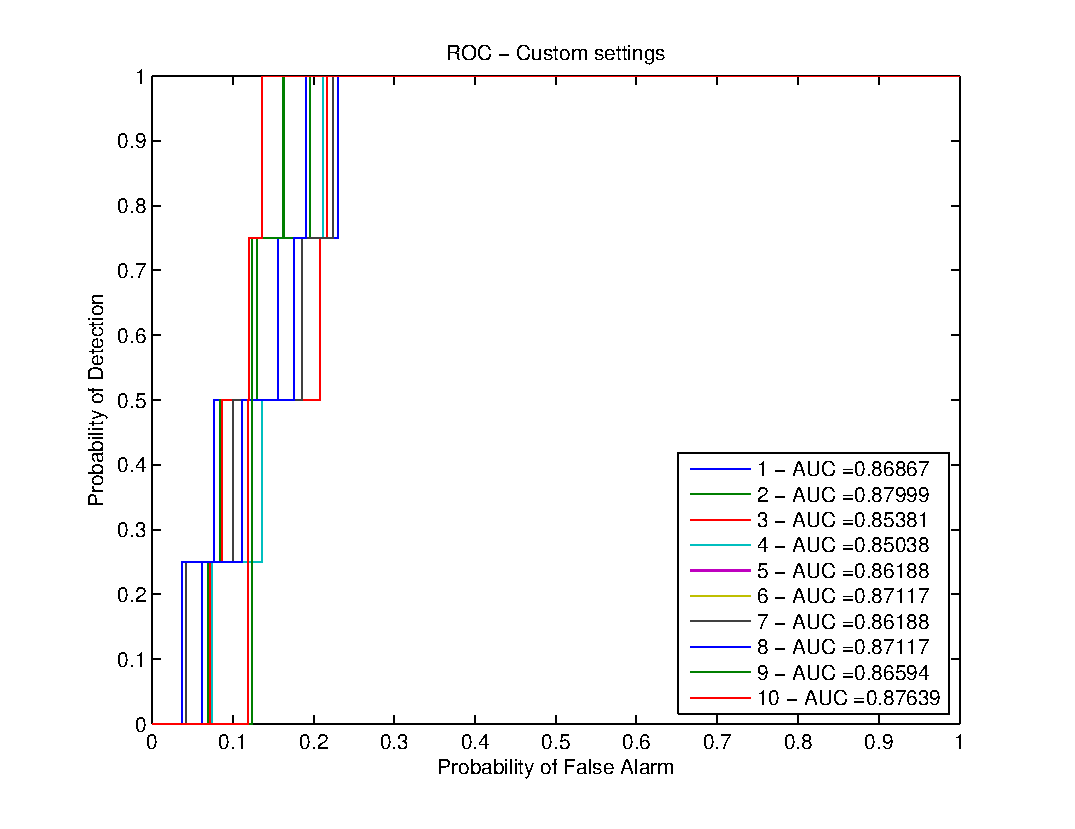
\includegraphics[width=0.9\linewidth]{k_sweep_2.eps}
  \caption{Result of comparing $k = 40$ and $k = 100$.}
  \label{fig:test:k:2}
\end{figure}

\begin{figure}
  \centering
  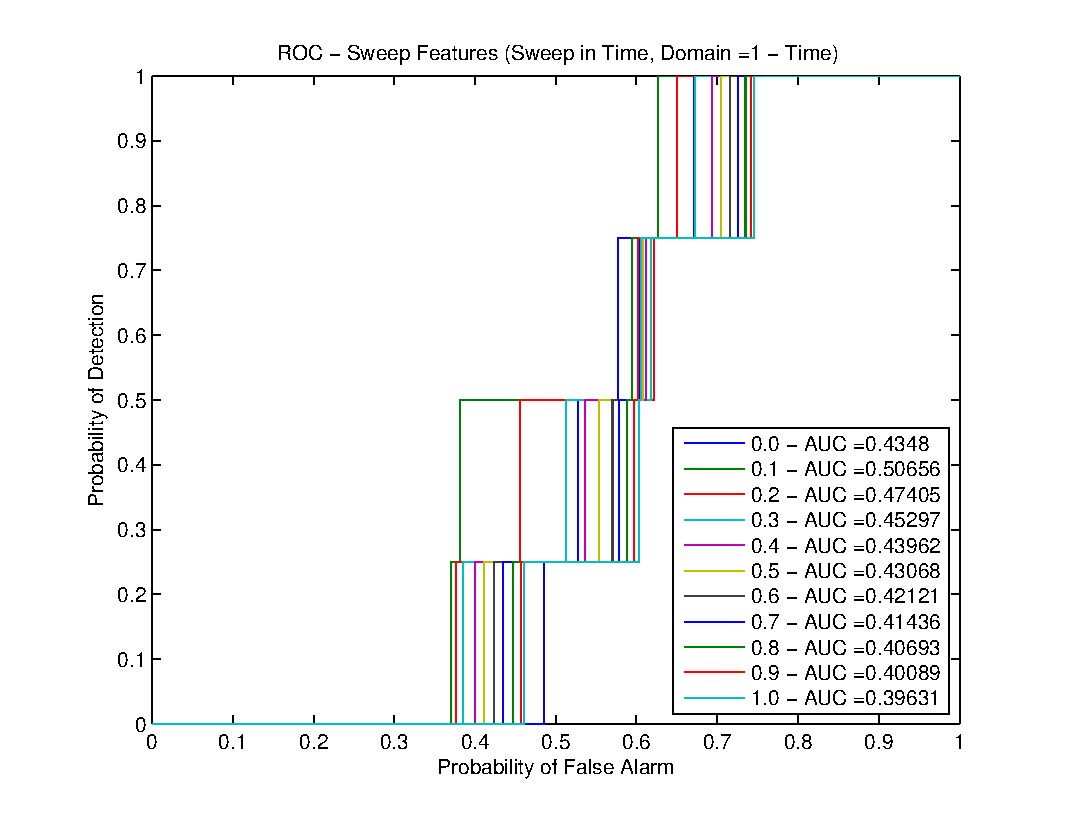
\includegraphics[width=0.9\linewidth]{weights.eps}
  \caption{Result of varying the weights for merging the graphs.}
  \label{fig:test:weights}
\end{figure}

\begin{figure}
  \centering
  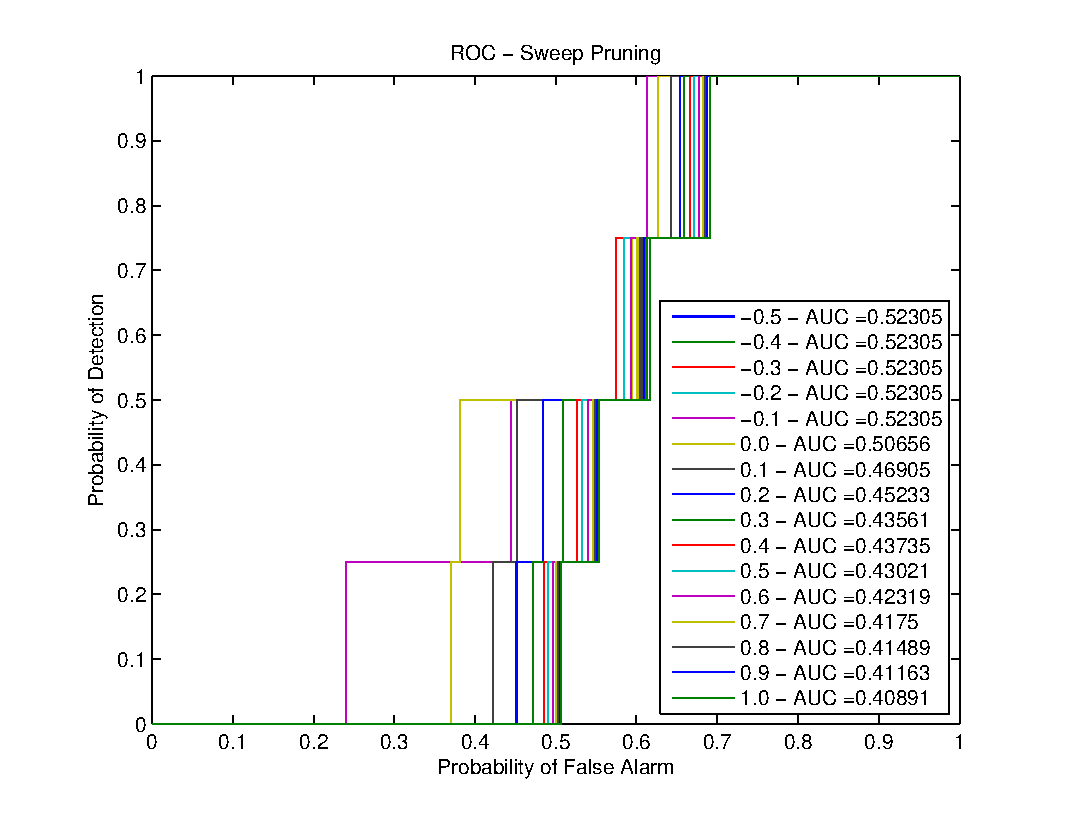
\includegraphics[width=0.9\linewidth]{pruning_sweep.eps}
  \caption{Result of varying the pruning threshold.}
  \label{fig:test:pruning}
\end{figure}

\begin{figure}
  \centering
  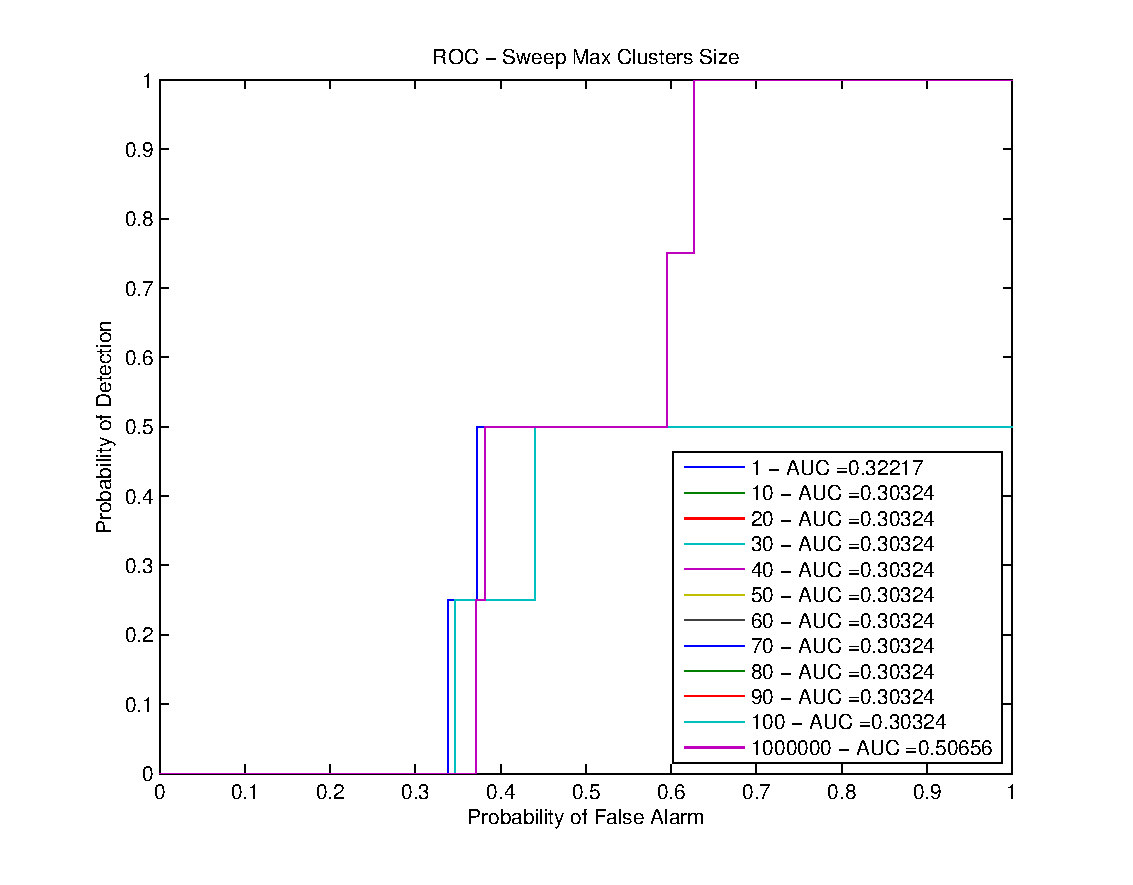
\includegraphics[width=0.9\linewidth]{clusters_sweep.eps}
  \caption{Result of varying the maximum cluster size.}
  \label{fig:test:cluster}
\end{figure}

\begin{figure}
  \centering
  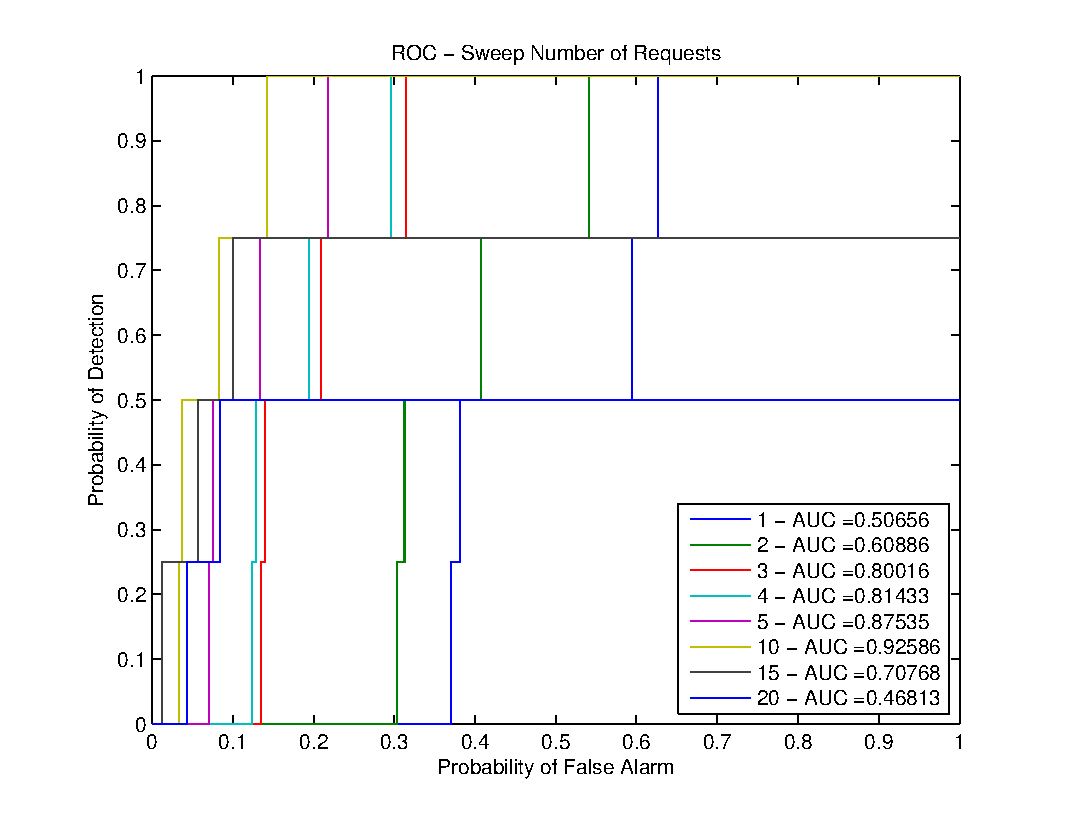
\includegraphics[width=0.9\linewidth]{requests_sweep.eps}
  \caption{Result of varying the minimum number of requests per client.}
  \label{fig:test:requests}
\end{figure}

\begin{figure}
  \centering
  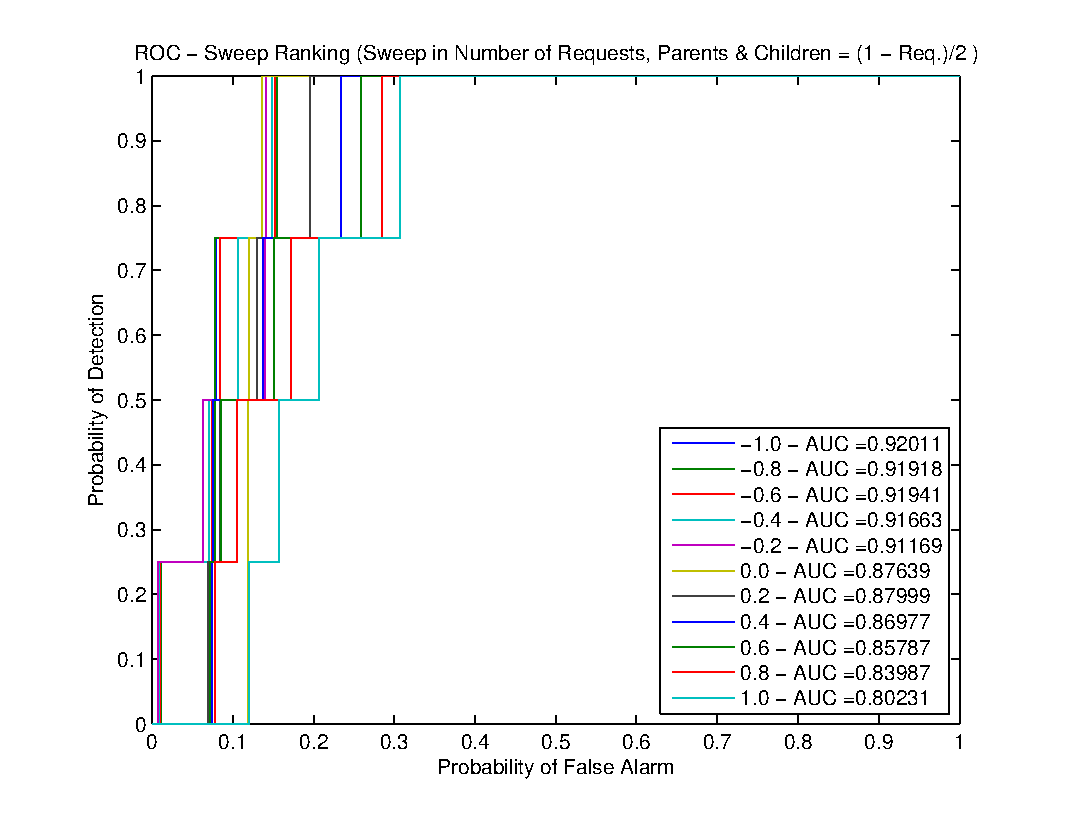
\includegraphics[width=0.9\linewidth]{ranking_sweep.eps}
  \caption{Result of varying the ranking weights.}
  \label{fig:test:ranking}
\end{figure}

\begin{figure}
  \centering
  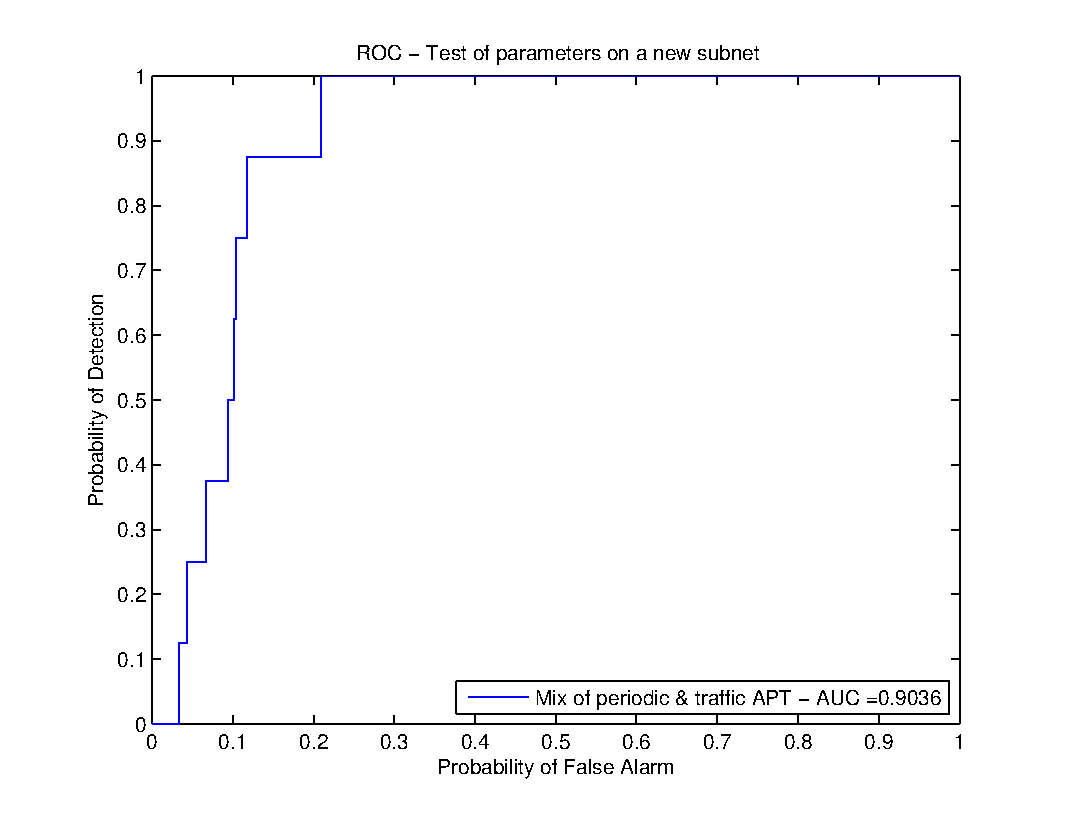
\includegraphics[width=0.9\linewidth]{cross_validation.eps}
  \caption{Result with a different dataset.}
  \label{fig:test:cross}
\end{figure}

\end{document}
